\subsection{Line picking on the rectangle with the Manhattan distance}
\label{sec:rect_manhattan}

The line-picking problem need not be considered one of ``straight''
lines. As discussed above, the general problem is one of determining
the distance between two randomly chosen points, where distance could
be determined by any valid metric.

In this case, we choose the points randomly on the rectangle (with
height $a$ and length $b$), but use the Manhattan distance (also
called the taxicab, or rectilinear, or L1 distance) between the two
points. Figure~\ref{fig:rect_man_eg} shows an example, illustrating
the rectilinear distance.

Figure~\ref{fig:rect_man_pdf} shows the PDF for one rectangle ($a=1$,
$b=2.5$). 


\begin{figure}[htbp]
  \begin{center}
    \subfloat[\label{fig:rect_man_eg}Example (with ratio 1:2.5).]
               {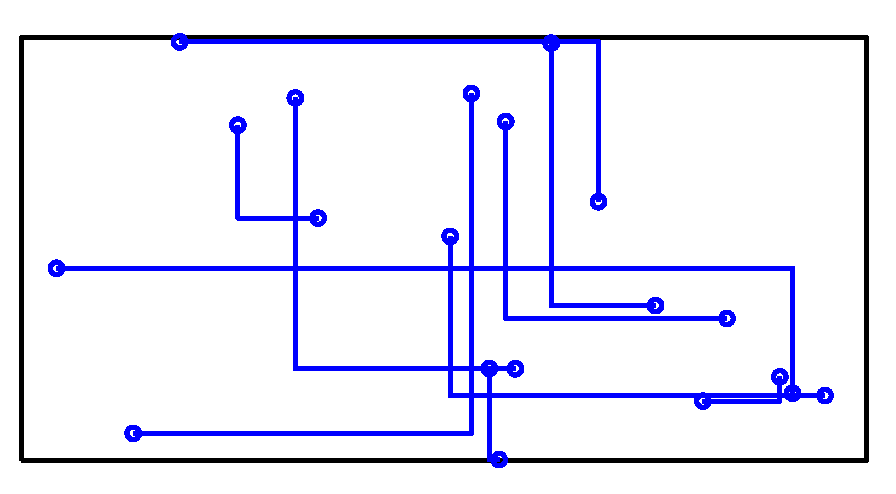
\includegraphics[width=0.3\columnwidth]
               {../Matlab/Plots/LinePicking_eg_rect_man.eps}} 
       \hspace{0.075\columnwidth}
    \subfloat[\label{fig:rect_man_pdf}PDF.]{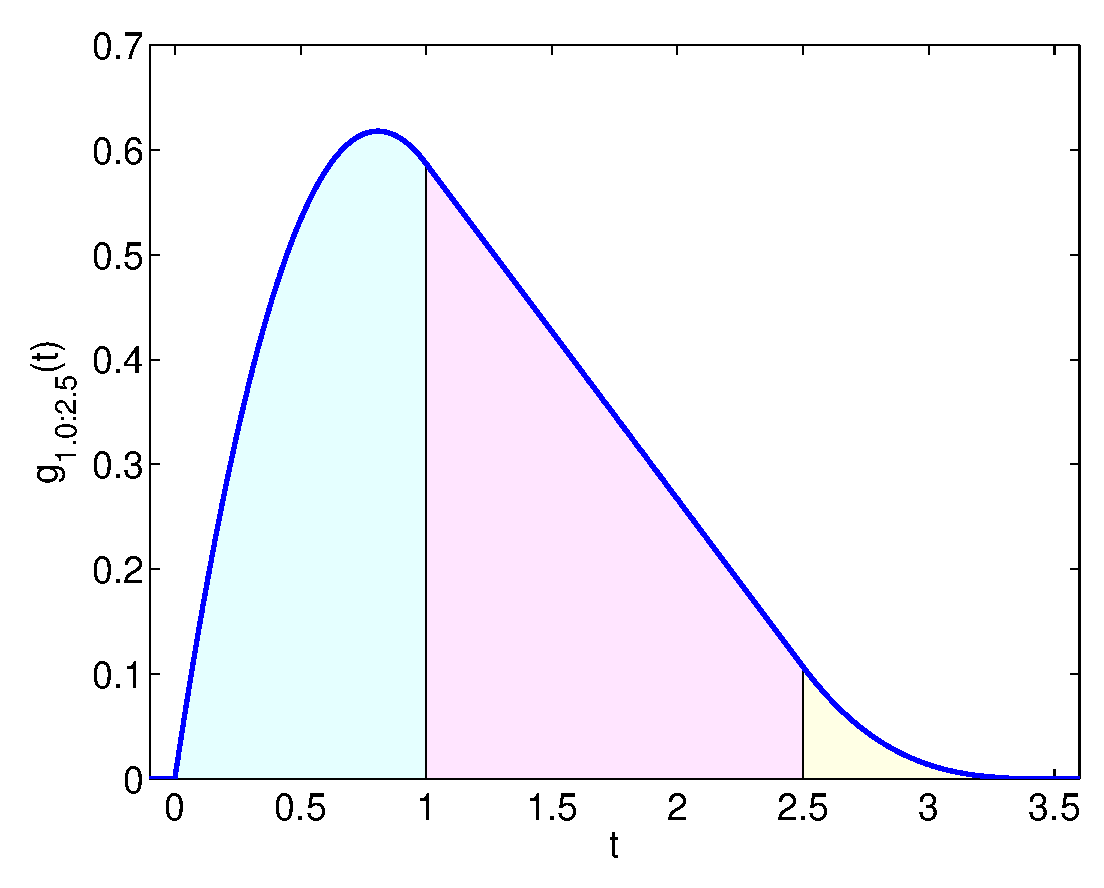
\includegraphics[width=0.5\columnwidth]
          {../Matlab/Plots/LinePicking_plot_rect_man_regions.eps}}
    \caption{The rectangle-line picking problem with Manhattan distance.}
  \end{center} 
\vspace{-4mm}
\end{figure}

\begin{table}[ht]
  \centering
  \begin{tabular}{|r|c|l|}
    \hline
    Statistic & Value & Source \\ 
    \hline
      Support            & $t \in [0, a+b]$ & \\
      PDF                & $ \displaystyle
 g^{\rm rect Man}_{a,b}(t) = \frac{2}{3 a^2 b^2} \times 
 \begin{cases}
 \displaystyle t \left(6 a b-3 a t-3 b t+t^2\right), & 0 \le t < a, \\
 \displaystyle a^2 (a+3 b-3 t),                      & a \le t <  b, \\
 \displaystyle (a+b-t)^3,                            & b \le t \le  a + b.\\
 \end{cases}
                             $ &
                             \eqref{eq:manhattan} \\
      CDF                &  & 
                             \eqref{eq:manhattan_cdf}\\
      $i$th Moment $m_i$ &  &
                             \eqref{} \\
      Mean               & $\displaystyle \frac{a+b}{3}$ &
                             \eqref{eq:rect_man_mean} \\
      Variance           & $\displaystyle  \frac{a^{2} + b^2}{18}$ &
                             \eqref{eq:rect_man_var} \\[1.5ex]
    \hline
  \end{tabular}
  \caption{Summary of the rectangle-line picking problem with Manhattan distance.}
  \label{tab:summary_rect_man}
\end{table}

\subsubsection{PDF}

The elegant feature of this problem is that the Manhattan distance is
made up from the horizontal distance, and the vertical distance, and
these two are independent. Hence the total distance is the sum of two
independent random variables, i.e.,
\[ t_{\rm Manhattan} = t_X + t_Y, \]
where $t_X$ and $t_Y$ are distances given by the line-line picking
problem (Section~\ref{sec:line_line}).

The probability density function of distances between two (uniformly)
randomly chosen points on the unit line is given in
\eqref{eq:line_line}, i.e., the densities in the $X$ and $Y$
directions for a rectangle with sides $a$ and $b$ will be $g^{\rm
  line}_b(t)$ and $g^{\rm line}_a(t)$.
% \begin{eqnarray}
%   \label{eq:rect_xy}
%   g^{\rm X}_b(t) & = & \left\{ \begin{array}{ll}
%                     \frac{2}{b} \left( 1-\frac{t}{b} \right), &
%                          \mbox{ for } 0 \leq t \leq b, \\
%                     0, & \mbox{ otherwise}, \\
%                   \end{array} \right. \nonumber \\
%   g^{\rm Y}_a(t) & = & \left\{ \begin{array}{ll}
%                     \frac{2}{a} \left( 1-\frac{t}{a} \right), &
%                          \mbox{ for } 0 \leq t \leq a, \\
%                     0, & \mbox{ otherwise}. \\
%                   \end{array} \right. \nonumber 
% \end{eqnarray}
The density for the Manhattan distance will be the convolution of
these, i.e., for $0 \leq t \leq a+b$, and $a \leq b$, we get
\begin{eqnarray}
    g^{\rm X+Y}_{a,b}(t) 
       & = & \left[ g^{\rm Y}_a *  g^{\rm X}_b \right] (t) \nonumber \\
\full{       & = & \int_{-\infty}^{\infty} g^{\rm Y}_a(s)  \, g^{\rm X}_b(t-s) \, ds,  \nonumber \\}
       & = & \int_{\max(0,t-b)}^{\min(a,t)} g^{\rm Y}_a(s)  \, g^{\rm X}_b(t-s) \, ds,  \nonumber \\
       & = & \frac{4}{a b} \int_{\max(0,t-b)}^{\min(a,t)}  
              \left( 1-\frac{s}{a} \right) 
              \left( 1-\frac{t-s}{b} \right)  \, ds,  \nonumber \\
\full{       & = & \frac{4}{a b} \int_{\max(0,t-b)}^{\min(a,t)} 
                   \left( 1 - \frac{t}{b} \right)  
                    + \left( \frac{1}{b} - \frac{1}{a} + \frac{t}{a b} \right)  s  
                    - \frac{1}{a b}  s^2 
                \, ds,  \nonumber \\}
       & = & \frac{4}{a b} \left[ \left( 1 - \frac{t}{b} \right) s
              + \frac{1}{2} \left( \frac{1}{b} - \frac{1}{a} + \frac{t}{a b} \right)  s^2 
              - \frac{1}{3} \frac{1}{a b}  s^3
                  \right]_{\max(0,t-b)}^{\min(a,t)},  \nonumber \\
\full{       & = & \left\{ \begin{array}{ll}
           \displaystyle
           \frac{4}{a b} \left( 1 - \frac{t}{b} \right) t
              + \frac{2}{a b} \left( \frac{1}{b} - \frac{1}{a} + \frac{t}{a b} \right)  t^2 
              - \frac{4}{3} \frac{1}{a^2 b^2}  t^3, & \mbox{ for } 0 \leq t \leq a, \\
           \displaystyle
           \frac{4}{a b}  \left( 1 - \frac{t}{b} \right) a
              + \frac{2}{a b} \left( \frac{1}{b} - \frac{1}{a} + \frac{t}{a b} \right)  a^2 
              - \frac{4}{3} \frac{1}{a^2 b^2}  a^3, & \mbox{ for } a \leq t \leq b, \\
           \displaystyle
             \frac{4}{a^2 b^2} \int_{0}^{a+b-t} 
                    u(a+b-t - u) \, du
                , & \mbox{ for } b \leq t \leq a + b , \\
                \end{array} \right. \nonumber \\}
       & = & \left\{ \begin{array}{ll}
           \displaystyle
           \left(\frac{4}{a b}\right) t
              - \left(\frac{2(a+b)}{a^2 b^2} \right) t^2
              + \left(\frac{2}{3} \frac{1}{a^2 b^2}\right)  t^3, & \mbox{ for } 0 \leq t \leq a, \\
           \displaystyle
                   \left( \frac{6b + 2a}{3b^2} \right)
              - \left( \frac{2}{b^2}  \right) t, & \mbox{ for } a \leq t \leq b, \\
           \displaystyle
              \frac{2(a+b-t)^3}{3 a^2 b^2}
                     , & \mbox{ for } b \leq t \leq a + b,  \\
           \displaystyle
             0, & \mbox{ otherwise}.
                \end{array} \right.
\end{eqnarray}
Which can be rearranged to give
\begin{equation}
 g^{\rm X+Y}_{a,b}(t) = \frac{2}{3 a^2 b^2} \times 
 \begin{cases}
 \displaystyle t \left(6 a b-3 a t-3 b t+t^2\right), & 0 \le t < a, \\
 \displaystyle a^2 (a+3 b-3 t),                      & a \le t <  b, \\
 \displaystyle (a+b-t)^3,                            & b \le t \le  a + b.\\
 \end{cases}
  \label{eq:manhattan}
\end{equation}

Figure~\ref{fig:rect_man_pdf_var} shows the PDFs for various
rectangles chosen such that $a + b = 1$ to allow comparison (the
choice means that the PDFs have the same support).

\begin{figure}[htbp]
  \begin{center}
    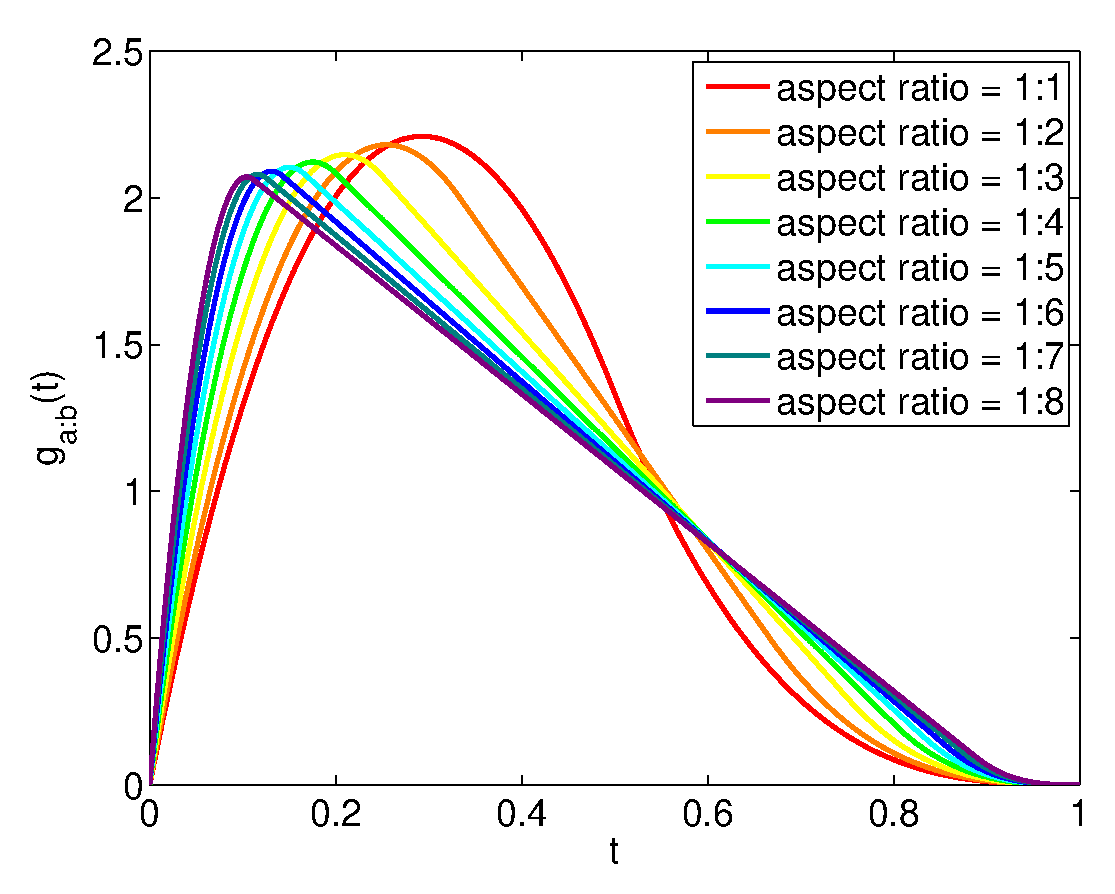
\includegraphics[width=0.55\columnwidth]
          {../Matlab/Plots/LinePicking_plot_rect_man.eps}
    \caption{The rectangle-line picking problem with Manhattan
      distance for various rectangles with $a+b = 1$.}
    \label{fig:rect_man_pdf_var}
  \end{center} 
\vspace{-4mm}
\end{figure}

\subsubsection{CDF}

The function above is comprised of several polynomial segments. A
closed form for the CDF is therefore easily derived (say by use of
Mathematica), but tiresome and not very instructive ...

Not so tiresome.., took less than typing in the paragraph above!!!
Especially if you use the method i did to get the PDF.

\begin{equation}
 G^{\rm X+Y}_{a,b}(t) =
 \begin{cases}
 0, & t \leq 0, \\
\frac{t^2 \left(-4 t (a+b)+12 a b+t^2\right)}{6 a^2 b^2}, & 0 \leq t \leq a, \\
-\frac{a^2+4 a (b-t)+6 t (t-2 b)}{6 b^2}, & a \leq t \leq  b, \\
-\frac{a^4+4 a^3 (b-t)+6 a^2 t (t-2 b)+4 a (b-t)^3+(b-t)^4}{6 a^2 b^2}, & b \leq t  \leq  a + b,\\
 1, & t \geq a + b.
 \end{cases}
  \label{eq:manhattan_cdf}
\end{equation}


\subsubsection{Moments}

As the $X$ and $Y$ distances are independent, we can form the mean and
variance as the sums of the means and variances of the line-line
picking problem, i.e.,
\begin{eqnarray}
  \mu^{\rm X+Y} & = & \frac{a+b}{3}, \\
  \label{eq:rect_man_mean}
  \sigma^2_{\rm X+Y}
      & = & \frac{a^{2} + b^2}{18}.
  \label{eq:rect_man_var}
\end{eqnarray}
